\documentclass[11pt]{beamer}
\usetheme{Warsaw}
\usepackage[utf8]{inputenc}
\usepackage[spanish]{babel}
\usepackage{amsmath,amsthm,amssymb} %modos matemáticos y  simbolos
\usepackage{latexsym,amsfonts} %simbolos matematicos
\usepackage{graphicx}
\usepackage{physics} %Simbolos fisicos
\usepackage{array} %mejores formatos de tabla
\usepackage{tabulary}
\usepackage{multirow} %ocupar varias filas en una tabla
\usepackage{fancybox} %recuadros talegas
\usepackage{float} %ubicar graficas
\usepackage{color}
\usepackage{comment}
\usepackage{stackrel}
\usepackage{calligra}
\usepackage{lipsum} % texto de relleno
\usepackage{cite}
\author{Diego Sarceño \\ \footnotesize{201900109}}
\title{Parcial 2 \\ \footnotesize{Materia Condensada 2}}
%\setbeamercovered{transparent} 
%\setbeamertemplate{navigation symbols}{} 
%\logo{} 
%\institute{} 
\date{\today} 
%\subject{} 
\begin{document}

\begin{frame}
\titlepage
\end{frame}

%\begin{frame}
%\tableofcontents
%\end{frame}

\frame{
	\frametitle{Capítulo 10 Problema 1 Enunciado}
	
	\onslide<1->{\textbf{Penetración de Campo Magnético en una placa. } La ecuación de penetración puede ser escrita como
		\begin{equation}
			\lambda ^2 \nabla ^2 B = B,  \label{london}
		\end{equation}
	donde $\lambda$ es la profundidad de penetración.}
	\begin{enumerate}[a)]
		\onslide<2->{\item Demuestre que $B(x)$ dentro de una placa superconductora perpendicular al eje $x$ y de grosor $\delta$ está dado por
			\begin{equation}
				B(x) = B_a \frac{\cosh{\flatfrac{x}{\lambda}}}{\cosh{\flatfrac{\delta}{2\lambda}}}, \label{bx}
			\end{equation}
		donde $B_a$ es el campo fuera de la placa y paralelo a ella; $x = 0$ es en el centro de la placa.}
		\onslide<3->{\item La magnetización efectiva $M(x)$ en la placa está definida por $B(x) - B_a = 4\pi M(x)$. Demuestre, en CGS, que $4\pi M(x) = -B_a (1/8\lambda ^2)(\delta ^2 - 4x^2)$, para $\delta \ll \lambda$.}
	\end{enumerate}

}


\frame{
	\frametitle{Capítulo 10 Problema 1 Solución}
	\onslide<1->{\textit{(a)} Tomando la ecuación \eqref{london} (Ecuación de London) y valuamos \eqref{bx}
		$$ \frac{\lambda ^2 B_a}{\cosh{\delta /2\lambda}} \underbrace{\pdv[2]{x} \cosh{x/\lambda}}_{\frac{1}{\lambda ^2} \cosh{x/\lambda}} = B_a \frac{\cosh{x/\lambda}}{\cosh{\delta /2\lambda}} $$}
	\onslide<2->{Lo que demuestra que cumple con la ecuación de London. \\}
	\onslide<3->{Ahora, dada la condición de frontera
		$$ B\qty(\pm \frac{\delta}{2}) = B_a , $$
		es claro que se cumple por la propiedad $\cosh{x} = \cosh{-x}$.} 
}









\frame{
	\frametitle{Capítulo 10 Problema 1 Solución}
	\onslide<1->{\textit{(b)} Para encontrar la magnetización efectiva y tomar en cuenta que $\lambda \gg \delta$, expandimos en taylor los cosenos hiperbólicos
		$$ \cosh{x/\lambda} = 1 + \frac{x^2}{2\lambda ^2} + \cdots $$
		$$ \cosh{\delta /2\lambda} = 1 + \frac{1}{2} \frac{\delta ^2}{4\lambda ^2} + \cdots . $$}
	\onslide<2->{Con esto, se toman los primeros términos y se sustituyen en la ecuación \eqref{bx}
		$$ B(x) = B_a \frac{1 + \frac{x^2}{2\lambda}}{1 + \frac{\delta ^2}{8\lambda ^2}} = B_a \frac{4(2\lambda ^2 + x^2)}{\delta ^2 + 8\lambda ^2}. $$}
	\onslide<3->{Reemplazamos esto en la definición de magnetización efectiva
		$$ 4\pi M(x) = B(x) - B_a = B_a \frac{4x^2 - \delta ^2}{\delta ^2 + 8\lambda ^2}, $$}
}




\frame{
	\frametitle{Capítulo 10 Problema 1 Solución}
	Ahora, para $\delta \ll \lambda$ se tiene $1/(\delta ^2 + 8\lambda ^2) \approx 1/8\lambda ^2$
		$$ 4\pi M(x) = -B_a \frac{1}{8\lambda ^2} \qty(\delta ^2 - 4x^2). $$
}





















\frame{
	\frametitle{Capítulo 16 Problema 3 Enunciado}
	\textbf{Efecto de un espacio de aire. } Discuta el efecto de un espacio de aire entre las placas de un capacitor y un dielectrico en la medición de constantes dieléctricas grandes. Cuál es la constante dieléctrica aparente más grande posible si el espacio de aire tiene un espesor de $10^{-3}$ del total del espesor? La presencia de espacios de aire pueden distorcionar la medición de constantes dieléctricas grandes.
	
	\begin{figure}[H]
		\centering
		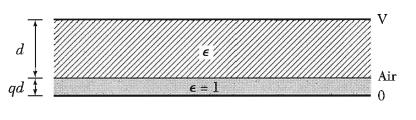
\includegraphics[scale=0.5]{./img/gap.png}
		\caption{Capacitor y dieléctricos.}
		\label{gap}
	\end{figure}
}







\frame{
	\frametitle{Capítulo 16 Problema 3 Solución}
		\onslide<1->{Dado que el desplazamiento eléctrico es continuo entre las superficies de un dieléctrico, entonces $E_{aire} = \varepsilon E_{diel}$. Dado esto podemos encontrar el potencial del dieléctrico
			$$ E_{aire} qd + E_{diel} d = E_{aire} d \qty(q + \frac{1}{\varepsilon}). $$}
		\onslide<2->{Por ley de Gauss $E_{aire} A = \flatfrac{Q}{\varepsilon _o} = 4\pi Q$, en CGS.}
		\onslide<3->{Para la capacitancia se tiene
			$$ C = \frac{A}{4\pi d\qty(q + \frac{1}{\varepsilon})}. $$}
		\onslide<4->{De la definición de capacitancia, podemos definir una constante dieléctrica 
		$$ \frac{1}{\varepsilon_e} = q + \frac{1}{\varepsilon}. $$}
}









\frame{
	\frametitle{Capítulo 16 Problema 3 Solución}
		Si hacemos a $\varepsilon$ muy grande para ver el comportamiento de $\varepsilon _e$, se tiene que para $\varepsilon \to \infty$
			$$ \varepsilon _e = \frac{1}{q}. $$
		Por lo que dicha constate dieléctrica no podrá tener un valor mas grande que $1/q = 10^3$.
}













\frame{
	\centering
	\vspace{1cm}
	GRACIAS POR SU ATENCIÓN $<3$
}














\end{document}